\documentclass[3p, authoryear, review]{elsarticle} %review=doublespace preprint=single 5p=2 column
%%% Begin My package additions %%%%%%%%%%%%%%%%%%%
\usepackage[hyphens]{url}

  \journal{Submitted to Transport Findings} % Sets Journal name


\usepackage{lineno} % add
\providecommand{\tightlist}{%
  \setlength{\itemsep}{0pt}\setlength{\parskip}{0pt}}

\usepackage{graphicx}
\usepackage{booktabs} % book-quality tables
%%%%%%%%%%%%%%%% end my additions to header

\usepackage[T1]{fontenc}
\usepackage{lmodern}
\usepackage{amssymb,amsmath}
\usepackage{ifxetex,ifluatex}
\usepackage{fixltx2e} % provides \textsubscript
% use upquote if available, for straight quotes in verbatim environments
\IfFileExists{upquote.sty}{\usepackage{upquote}}{}
\ifnum 0\ifxetex 1\fi\ifluatex 1\fi=0 % if pdftex
  \usepackage[utf8]{inputenc}
\else % if luatex or xelatex
  \usepackage{fontspec}
  \ifxetex
    \usepackage{xltxtra,xunicode}
  \fi
  \defaultfontfeatures{Mapping=tex-text,Scale=MatchLowercase}
  \newcommand{\euro}{€}
\fi
% use microtype if available
\IfFileExists{microtype.sty}{\usepackage{microtype}}{}
\usepackage{natbib}
\bibliographystyle{plainnat}
\usepackage{longtable}
\usepackage{graphicx}
% We will generate all images so they have a width \maxwidth. This means
% that they will get their normal width if they fit onto the page, but
% are scaled down if they would overflow the margins.
\makeatletter
\def\maxwidth{\ifdim\Gin@nat@width>\linewidth\linewidth
\else\Gin@nat@width\fi}
\makeatother
\let\Oldincludegraphics\includegraphics
\renewcommand{\includegraphics}[1]{\Oldincludegraphics[width=\maxwidth]{#1}}
\ifxetex
  \usepackage[setpagesize=false, % page size defined by xetex
              unicode=false, % unicode breaks when used with xetex
              xetex]{hyperref}
\else
  \usepackage[unicode=true]{hyperref}
\fi
\hypersetup{breaklinks=true,
            bookmarks=true,
            pdfauthor={},
            pdftitle={The Effect of Transit Signal Priority on Bus Rapid Transit Headway Adherence},
            colorlinks=false,
            urlcolor=blue,
            linkcolor=magenta,
            pdfborder={0 0 0}}
\urlstyle{same}  % don't use monospace font for urls

\setcounter{secnumdepth}{5}
% Pandoc toggle for numbering sections (defaults to be off)


% Pandoc header
\usepackage{booktabs}
\usepackage{booktabs}
\usepackage{longtable}
\usepackage{array}
\usepackage{multirow}
\usepackage{wrapfig}
\usepackage{float}
\usepackage{colortbl}
\usepackage{pdflscape}
\usepackage{tabu}
\usepackage{threeparttable}
\usepackage{threeparttablex}
\usepackage[normalem]{ulem}
\usepackage{makecell}
\usepackage{xcolor}



\begin{document}
\begin{frontmatter}

  \title{The Effect of Transit Signal Priority on Bus Rapid Transit Headway Adherence}
    \author[BYU]{Gregory Macfarlane\corref{1}}
   \ead{gregmacfarlane@byu.edu} 
    \author[BYU]{Grant Schultz}
   \ead{gschultz@byu.edu} 
    \author[WCG]{Michael Sheffield}
   \ead{michael.sheffield@wcg.us} 
    \author[BYU]{Logan Bennett}
   \ead{loganbennett93@gmail.com} 
      \address[BYU]{Brigham Young University, Civil and Environmental Engineering Department, 430 Engineering Building, Provo, Utah 84602}
    \address[WCG]{Wall Consultant Group, 9980 S 300 W Ste 200 Sandy, UT 84070}
      \cortext[1]{Corresponding Author}
  
  \begin{abstract}
  We report the results of an experiment to evaluate the impact of transit signal priority (TSP) on headway adherence for a bus rapid transit (BRT) system in Provo / Orem, Utah. The system grants TSP if the bus is running behind its unpublished schedule, but users perceive only a headway. In general, we find that more permissive TSP regimes modestly but significantly reduce the 85th percentile headway, controlling for directionality and time period. An inconsistent result gives that a strict TSP regime has a higher 85th percentile headway than not using TSP at all.
  \end{abstract}
   \begin{keyword} Public transit, Transit signal priority, Traffic operations\end{keyword}
 \end{frontmatter}

\hypertarget{intro}{%
\section{Questions}\label{intro}}

Transit signal priority (TSP) allows traffic signals to flexibly accommodate
transit vehicles. This may involve extending a green phase until the vehicle
passes, triggering an early green if there is a vehicle waiting at the light, or
even running specific transit-only phases. TSP helps transit vehicles maintain
on-time performance \citep{Liu2018}, but often TSP will only engage at a signal if
the vehicle is running behind its schedule, thus minimizing automobile delay
when the bus is otherwise on schedule \citep{NI20201}.

In 2018, the Utah Transit Authority (UTA) launched the Utah Valley Express (UVX)
Bus Rapid Transit (BRT) system in Provo and Orem, Utah. The system connects
two commuter rail stations, two major universities (Brigham Young and Utah Valley),
and commercial districts in Orem and Provo. UVX has TSP on X of the X traffic
signals along its route. The TSP is triggered when a vehicle is behind its schedule;
however, the system does not publish a schedule and rather attempts to maintain
a specific headway (6 minutes in the peak period and 10 minutes in the off-peak).

The research questions are therefore:

\begin{itemize}
\tightlist
\item
  Does schedule-based TSP improve headway adherence for rapid transit systems?
\item
  Is there an average improvement, or is there a reduction in extreme delay?
\item
  Is there an improvement difference by time of day or for particular portions
  of a rapid transit route?
\end{itemize}

\hypertarget{methods}{%
\section{Methods}\label{methods}}

UTA provided timepoint data for all trips on the UVX system for the entirety of
2019. We calculated the headway between successive UVX trips at each stop, as
well as the cumulative dwell time of all stations along the route. Because the
UVX route loops around south Provo and stops at the Provo FrontRunner station
twice, this created some minor difficulties in data processing, and we removed
the timepoints on this portion of the route. We also limit our analysis to the
period between 7 AM and 8 PM.

From January through June 6, the system operated with a 5-minute TSP threshold,.
with TSP granted only if the vehicle was five or more minutes behind its
scheduled timepoint. After August 12, the system switched to a 2-minute TSP
threshold. During the summer, the TSP system was configured as follows for this
experiment:

\begin{itemize}
\tightlist
\item
  May 2 through June 6, 2019: 5 minute threshold
\item
  June 10 through July 12 and after August 12: 2 minute threshold
\item
  July 15 through July 26: no TSP
\item
  July 30 through August 9: TSP always activated
\end{itemize}

We discarded trips from January through April and September through December
because the additional university passenger demand could interfere in the
experiment and there were no tests of the ``None'' or ``Always'' TSP thresholds
during the school year.

Standard statistical tests --- such as the student's \(t\)-test or
ordinary least squares regression models --- are designed to ascertain the
significance of a statistic at the \emph{mean} of the distribution. In this
application, we are less concerned with the mean deviation in headway, and are
instead interested in whether TSP is able to reduce the lateness of buses that
already have substantial deviation from their programmed headway. Consequently,
we employ conditional quantile regression \citep{koenker2001quantile} to estimate the
effect of TSP on headway deviation at the 85th percentile of the distribution.
This is done with the \texttt{quantreg} package for R \citep{quantreg, R}

\hypertarget{findings}{%
\section{Findings}\label{findings}}

Figure \ref{fig:ecdf} shows the empirical cumulative density function for the
headway deviation data, grouped by TSP threshold. Visually, the difference
between the various threshold settings is not dramatic. The 5-minute
threshold appears to have slightly more vehicles arrive ahead of the
scheduled headway, and slightly fewer arrive behind it, than the other three
threshold groups. The median and average of the distribution for all four
thresholds is remarkably similar, and strengthens our determination to
examine the edges of the distribution with a quantile regression model.

\begin{figure}
\centering
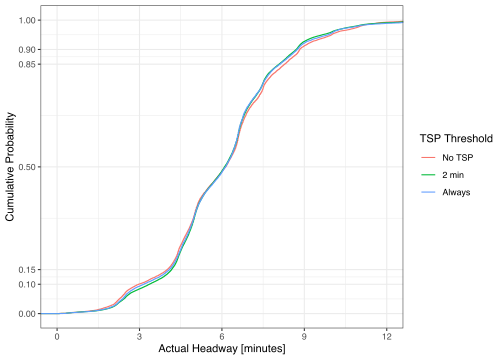
\includegraphics{uvx_headways_files/figure-latex/ecdf-1.pdf}
\caption{\label{fig:ecdf}Cumulative probability distribution of headway deviation by threshold.}
\end{figure}

\begin{table}

\caption{\label{tab:models}85th Percentile Regression Estimates}
\centering
\begin{tabular}[t]{lcccc}
\toprule
  & Threshold & Direction & Peak & All\\
\midrule
(Intercept) & 2.067 (46.600)*** & 1.683 (65.528)*** & 1.967 (57.740)*** & 1.650 (68.493)***\\
TSP: 5 minutes & 0.300 (5.846)*** & 0.200 (6.113)*** & 0.233 (5.853)*** & 0.167 (5.579)***\\
TSP: 2 minutes & -0.117 (-2.467)** & -0.067 (-2.433)** & -0.117 (-3.569)*** & -0.083 (-3.366)***\\
TSP: Always & -0.100 (-1.800)* & -0.083 (-2.430)** & -0.100 (-2.562)** & -0.100 (-2.849)***\\
Southbound &  & 0.917 (42.553)*** &  & 0.883 (27.572)***\\
AM Peak &  &  & -0.050 (-2.284)** & 0.000 (0.000)\\
PM Peak &  &  & 0.617 (21.248)*** & 0.533 (11.790)***\\
Southbound \$\textbackslash{}times\$ AM Peak &  &  &  & -0.067 (-1.282)\\
Southbound \$\textbackslash{}times\$ PM Peak &  &  &  & -0.183 (-2.757)***\\
\midrule
AIC & 760,763.5 & 755,372.3 & 759,075.1 & 754,484.1\\
Log Likelihood & -380,377.8 & -377,681.1 & -379,531.6 & -377,233\\
\bottomrule
\multicolumn{5}{l}{\textsuperscript{} t-statistics in parentheses}\\
\multicolumn{5}{l}{\textsuperscript{} * p $<$ 0.1, ** p $<$ 0.05, *** p $<$ 0.01}\\
\end{tabular}
\end{table}

Table \ref{tab:models} presents the estimates of four models with an array
of explanatory variables. In the model labeled ``Threshold,'' each TSP threshold
is controlled for with a dummy variable; the intercept term suggests that the
85th percentile bus arrives with a headway 2.0666667
minutes longer than it was supposed to have. The three threshold dummies are
each significant, though the ordering of the coefficients is somewhat unintuitive.
Relative to the situation with no TSP, making TSP always available reduces the
headway of the 85th percentile bus by 0.1
minutes, and engaging TSP at a 2-minute threshold reduces the headway by
0.1166667. What is not intuitive is that
engaging TSP with a 5-minute threshold actually makes the 85th percentile
headway -0.3 minutes \emph{longer} than
not using it at all.

The other three models in Table \ref{tab:models} control for the direction
of the service (southbound buses from Orem to Provo have a longer headway), the
time period (operating in the PM peak lengthens the headway), and an interaction
term between those two variables. With each additional control, the central
findings related to TSP are unchanged in either magnitude or significance.

The finding that a 5-minute TSP threshold appears to lengthen the headway
relative to not using TSP at all is curious, and we cannot immediately
account for it. The schedule of threshold changes was not randomized in any way,
and it is possible that the results of this study are tied up in unaccounted
seasonal variations. In spite of this curious finding, we find that --- all else
equal --- TSP marginally improves the headway adherence of late-running BRT
vehicles.

\bibliography{book.bib}


\end{document}

